\section{Phân tích Thiết kế hệ thống}

\subsection{User Stories}
\textbf{User Story về giao diện trò chơi:}
\begin{itemize}
	\item Là một Game Player, tôi muốn trò chơi chơi ở toàn màn hình.
	\item Là một Game Player, tôi muốn trò chơi chơi ở nhiều tỉ lệ khác nhau.
	\item Là một Game Player, tôi muốn menu có các nút đơn giản dễ sử dụng.
	\item Là một Game Player, tôi muốn giao diện trang bị trực quan, tôi có thể xem thông tin trang bị, cũng như sắp xếp và di chuyển trang bị từ khung trang bị vào kho đồ và ngược lại.
	\item Là một Game Player, tôi muốn giao diện bên ngoài màn chơi trực quan, các mục được hiện rõ ràng và dễ thao tác
	\item Là một Game Player, tôi muốn giao diện khi chiến đấu rõ ràng, các nút bấm dễ nhìn.
	\item Là một Game Player, tôi muốn giao diện bảng trả về trực quan, hiện đầy đủ thông tin, cũng như tôi có thể xem toàn bộ nội dung trong cell.
	\item Là một Game Player, tôi muốn player có thể hiển thị thông tin về tình trạng hiện tại, trang bị hiện có, những thông tin phải được cập nhật liên tục để tôi có thể xử lý các nước đi tiếp theo.
	\item Là một Game Player, tôi muốn có một hệ thống tab để tôi có thể chuyển đổi qua lại giữa các tab bảng trả về. 
	\item Là một Game Player, tôi muốn có hệ thống cài đặt cho phép cài đặt âm thanh, hình ảnh của trò chơi.
	\item Là một Game Player, tôi muốn có một phần để hiển thị thông tin của nhà phát triển.
	\item Là một Game Player, tôi muốn có một nút để thoát trò chơi.
	\item Là một Game Player, tôi muốn có nhiều người dùng được lưu trong game, mỗi người dùng sẽ có tên người chơi. Tôi có thể đổi được tên, thêm, xoá người dùng.
\end{itemize}
\textbf{User Story về cơ chế chơi:}
\begin{itemize}
	\item Là một Game Player, tôi muốn có nhiều màn chơi, chia thành nhiều Chapter để dễ theo dõi. Mỗi màn chơi sẽ hướng dẫn tôi những cơ chế mới của trò chơi với độ khó tăng dần.
	\item Là một Game Player, tôi muốn giao diện màn chơi đơn giản, dễ nhìn.
	\item Là một Game Player, tôi muốn trò chơi có phong cách đồ hoạ Fantasy, những nhân vật được nhân hoá.
	\item Là một Game Player, tôi muốn tôi có thể chèn, xoá, cập nhật các bảng trong schema tự do mà không bị lỗi.
	\item Là một Game Player, tôi muốn game có một sự phản hồi sau khi tôi nhập câu lệnh và chạy.
	\item Là một Game Player, tôi muốn player sẽ có một số phản ứng khi tôi nhập các câu lệnh nhất định (như attack hay use).
	\item Là một Game Player, tôi muốn trong màn chơi có hiển thị rõ các yêu cầu của màn chơi.
	\item Là một Game Player, tôi muốn sau khi bảng kết quả truy vấn hiện ra, tôi có thể xem toàn bộ nội dung của cell, sao chép nội dung đó hoặc sao chép toàn bộ hàng của bảng đó.
	\item Là một Game Player, tôi muốn có một nơi để tôi có thể ghi lại các ghi chú, gợi ý, hoặc dán nội dung đã sao chép từ bảng dữ liệu ra.
	\item Là một Game Player, tôi muốn có các animation cho các vật thể tương ứng với các hành động khác nhau, như idle, running, attacking,...
	\item Là một Game Player, trong trường hợp tôi nhập sai câu lệnh, hệ thống sẽ báo lỗi tôi sai như thế nào và tôi có thể chỉnh sửa lại câu lệnh sau cho đúng. 
	\item Là một Game Player, tôi muốn xem schema diagram, bản đồ của màn chơi.
	\item Là một Game Player, tôi muốn có một documentation về ngôn ngữ SQL và có một nút hiển thị để tôi có thể thuận tiện tra cứu.
	\item Là một Game Player, tôi muốn có một nút tạm dừng trò chơi, cũng như có thể save lại tiến trình màn chơi của tôi.
	\item Là một Game Player, tôi muốn tôi có thể chơi xuyên suốt toàn bộ màn chơi mà không gặp sự ngắt ngang bởi các yếu tố như quảng cáo,...
	\item Là một Game Player, sau khi hoàn thành màn chơi, tôi muốn một bảng hiện kết quả màn chơi kèm các nút bấm để di chuyển nhanh giữa các màn chơi.
\end{itemize}



\subsection{Các yêu cầu của hệ thống}
\subsubsection{Yêu cầu chức năng}
\paragraph {Yêu cầu chức năng liên quan đến giao diện trò chơi}
\begin{itemize}
	\item Trò chơi sẽ chơi ở chế độ toàn màn hình.
	\item Giao diện trang bị trực quan, chia làm 3 phần: Kho đồ, slot trang bị và thông số người chơi. Có thể dùng chuột để xem thông tin trang bị, cũng như sắp xếp và di chuyển trang bị từ khung trang bị vào kho đồ và ngược lại.
	\item Giao diện bên ngoài màn chơi gồm bản đồ để chọn mà chơi. Thông tin màn chơi sẽ được hiện lên khi người chơi di chuột đến, cùng với các nút để mở giao diện trang bị và để vào shop để mua bán vật phẩm.
	\item Menu của trò chơi gồm có các nút bấm: Play để bắt đầu chơi; Setting để người chơi thiết lập cài đặt trò chơi; Help để hiện giao diện hướng dẫn; Credit để hiển thị thông tin nhà phát hành; Exit để thoát trò chơi.
	\item Trò chơi có giao diện chuyển đổi người dùng, người chơi có thể thêm, xoá người dùng có phần để hiển thị tên của người chơi. Người chơi có thể tự do thay đổi tên.
\end{itemize}


\paragraph{Yêu cầu chức năng liên quan đến giao diện màn chơi}
\begin{itemize}
		\item Giao diện màn chơi được phân chia rõ ràng các khu vực
		\begin{itemize}
			\item Vùng giao diện bên dưới chứa các tab là kết quả trả về của các câu truy vấn \textbf{select}, các nút điều hướng tabs, thanh nhập câu lệnh và vùng để chứa thông tin người chơi. Giao diện bảng record trực quan, các cell dễ nhìn, có thể xem được toàn bộ nội dung cũng như có thể sao chép toàn bộ nội dung của cell, cũng như cũng có thể sao chép toàn bộ hàng. Ngoài ra Có một vùng để điều hướng sang các tab khác, mỗi tab là kết quả bảng trả về, ngoài ra còn có tab Notes cho người chơi ghi các ghi chú trong quá trình chơi. Vùng Player trên giao diện có thể hiển thị thông tin về tình trạng hiện tại, trang bị hiện có, những thông tin phải được cập nhật liên tục để người chơi có thể xử lý các nước đi tiếp theo.
			\item Vùng giao diện bên trên chứa thông tin màn chơi và các nút chức năng.
			\item Vùng chiến đấu, phía bên trái hiện tên người chơi và số máu còn lại. Phía bên phải hiện tên quái vật và số bộ phần còn lại của quái vật. Cả hai bên đều có hiển thị trạng thái hiệu ứng hiện tại của mỗi thực thể đang chiến đấu
		\end{itemize}
		\item Khi gây sát thương, cần có dòng văn bản hiển thị số sát thương mà nhân vật tấn công gây ra cho đối phương (có thể tuỳ từng loại). Sau khi kết thúc đòn đánh, có thể có một hộp thoại thông báo tính hiệu quả đòn đánh, xem đòn đánh có "Effective" hay không,...
		\item Có hộp thoại chứa schema diagram và bản đồ của màn chơi, giúp người chơi tra cứu.
		\item Có hộp thoại documentation về ngôn ngữ SQL để người chơi tham khảo.
	
\end{itemize}


\paragraph{Yêu cầu chức năng liên quan đến cơ chế chơi}
\begin{itemize}
	\item Chế độ cốt truyện được chia thành nhiều màn chơi, chia thành các Chapter cho mỗi khu vực lớn trên bản đồ. Mỗi màn chơi sẽ hướng dẫn những cơ chế mới của trò chơi với độ khó tăng dần. Càng đi sâu trong màn chơi độ khó sẽ tăng dần. 
	\item Người chơi có thể chèn, xoá, cập nhật các bảng trong schema tự do mà không bị lỗi, trừ một số bảng đặc biệt. Đặc biệt là vùng chiến đấu, với các phản ứng của câu lệnh thì vùng chiến đấu sẽ có những hiển thị nhất định để cho người chơi thấy được những gì đã xảy ra sau khi người chơi chạy câu truy vấn.
	\item Các nhân vật có hoạt hình chuyển động, khi đang đợi lượt đi, khi tấn công, sử dụng vật phẩm, khi bị tấn công và khi bị tiêu diệt.
	\item Vùng chiến đấu hiển thị cấc thông tin về quái vật, về các phản ứng đòn đánh, về ngoại hình, hộp thoại cần được hiển thị chính xác để người chơi xác định đúng mục tiêu.
	\item Trong trường hợp người chơi nhập câu lệnh có lỗi ở mức SQL, hệ thống sẽ báo lỗi câu truy vấn sai như thế nào và sẽ không kết thúc lượt của người chơi, người chơi có thể chỉnh sửa lại sao cho đúng. 
	\item Cần có sự cân bằng trong game ở tất cả khía cạnh. Không thể để xảy ra trường hợp Over Powered (quá mạnh) hoặc Under Powered (quá yếu),...
	\item Cần xử lý các trường hợp người chơi cố tình thay đổi cấu trúc schema, chèn, update và xoá record trong bảng nhằm mục đích phá hoại, làm game bị lỗi và không thể hoạt động được nữa.
	\item Khi hoàn thành màn chơi, một bản thông báo sẽ xuất hiện. Bảng này hiển thị các thử thách đã đạt được và 3 nút bấm. Một nút bấm để trở về lựa chọn màn chơi, một nút bấm để chơi lại và một nút bấm để đến màn chơi kế tiếp.
	
\end{itemize}


\subsubsection{Yêu cầu phi chức năng}

\textbf{Yêu cầu phi chức năng liên quan đến Game Player:}
\begin{itemize}
	\item Hiệu năng ổn định, có thể chạy với 60FPS trong các ngữ cảnh khác nhau với cấu hình i5 - 8265U, Card Nvidia MX150, 12GB RAM. Có thể chạy với 120FPS khi tinh chỉnh cài đặt về đồ hoạ trên các cấu hình cao hơn.
	\item Giao diện của trò chơi nên đơn giản, dễ hiểu, phù hợp với nhiều loại người chơi. Cần tránh các thao tác rườm rà, phức tạp.
	Người chơi có thể thành thục chơi sau 30 phút trải nghiệm
	\item Phong cách đồ hoạ 2D Pixel, sử dụng các hiệu ứng kỹ xảo để đánh bóng game.
	\item Game giữ được sự ổn định khi quy mô của các object tăng lên, với nhiều object trong màn chơi ngày càng nhiều, hiệu ứng ngày càng dày đăc mà không có sự sụt giảm về hiệu năng.
	\item Game nên chạy mượt mà không gặp vấn đề lớn về bug, glitch. Hệ thống save load hoạt động hiệu quả, có thể lưu lại tiến trình màn chơi, kể cả khi tắt ngang trò chơi, hoặc sự cố về phần mềm như crash, sự cố về phần cứng và hệ điều hành.
	\item Các màn chơi cần có độ khó tăng dần, xoay tua giữa việc giới thiệu các tính năng mới và luyện tập các tính năng đã học. Màn chơi phải có độ khó vừa phải, không quá khó cũng không quá dễ.
	\item Thời gian phản ứng sau khi thực hiện câu truy vấn thấp, nhỏ hơn 1 giây. Sau khi chạy phải có kết quả trả về tương ứng với loại câu truy vấn.
\end{itemize}
\subsection{Usecase Diagram của Game}
\begin{figure}[H]
	\centering
	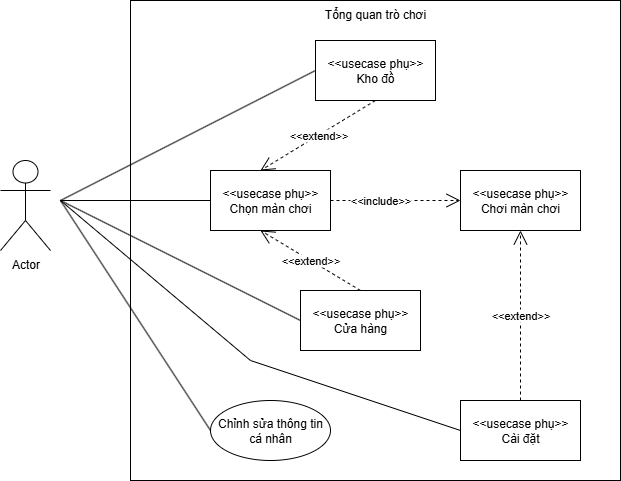
\includegraphics[width=14cm]{Images/overallUCD.png}
	\vspace{0.5cm}
	\caption{Usecase Diagram Tổng quan của Game}
\end{figure}

\hspace*{0.5cm} Người chơi có thể chỉnh sửa thông tin cá nhân của người chơi như tên, mô tả,... Ngoài ra còn có một số chức năng khác được quy định trong các use-case phụ như sau:
\begin{itemize}
	\item Chọn màn chơi: người chơi được đưa đến use-case chọn màn chơi, use-case chỉ ra người chơi có thể làm gì trong đó.
	\item Chơi màn chơi: người chơi sẽ được đưa đến use-case màn chơi, use-case màn chơi chỉ ra người chơi có thể làm được gì trong màn chơi đó.
	\item Kho đồ: khi người chơi mở kho đồ từ màn hình chọn màn chơi, người chơi sẽ được đưa tới use-case kho đồ, nơi người chơi có thể thao tác với kho đồ và trang bị của mình.
	\item Cửa hàng: khi người chơi mở cửa hàng từ màn hình chọn màn chơi, người chơi sẽ được đưa tới use-case cửa hàng, nơi người chơi có thể thực hiện các thao tác buôn bán vật phẩm, trang bị.
	\item Cài đặt: Use-case phụ này mô tả các khả năng của người chơi khi truy cập vào cài đặt, bao gồm điều chỉnh các thông số của trò chơi.
\end{itemize}

\subsubsection{Kho đồ}
Use-case cho chức năng kho đồ
\begin{figure}[H]
	\centering
	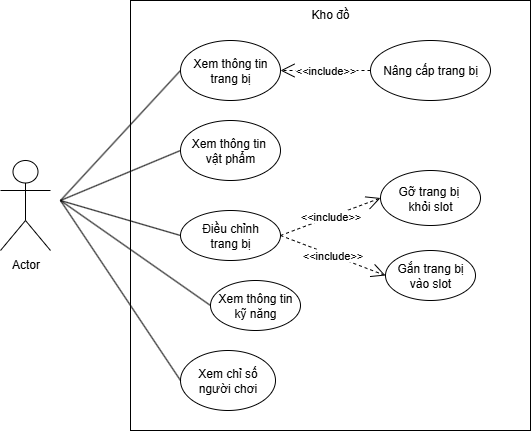
\includegraphics[width=14cm]{Images/InventoryUCD.png}
	\vspace{0.5cm}
	\caption{Usecase Diagram Kho đồ của Game}
\end{figure}
\begin{center}
	\begin{tabular}{|l|p{12cm}|}
		\hline
		ID and Name & UC1: Kho đồ \\
		\hline
		Actor  & Người chơi \\
		\hline
		Description  & Use-case này chỉ các khả năng người chơi khi truy cập trang kho đồ\\
		\hline
		Trigger  & Người chơi nhấn chuột trái vào nút mở Kho đồ.\\
		\hline
		Pre-conditions & Người chơi hiện đang ở màn hình chính hoặc ở màn hình chọn màn chơi\\
		\hline
		Post-conditions & Người chơi gắn hoặc gỡ trang bị khỏi kho đồ, hoặc đã thực hiện nâng cấp xong\\
		\hline
		\multirow{2}{*}{Normal flow}      &\qquad 1.Người chơi xem thông tin của món vật phẩm hoặc trang bị, bao gồm cấp hiện tại (đối với trang bị), hoặc số lượng đối với (các vật phẩm khác).\\
		&\qquad 2. Người chơi ấn vào trang bị trong kho đồ, chọn Gắn trang bị (hoặc kéo thả vào ô trang bị mong muốn)\\
		&\qquad 3. Người chơi ấn Đóng, kết thúc usecase kho đồ\\
		\hline
		Alternative flow  & \qquad A1. Tại bước 1, người chơi xem thông tin của trang bị, người chơi có thể nâng cấp trang bị với một xác suất thành công nhất định. Sau khi báo kết quả người chơi được về đầu bước số 1\\
		&\qquad A2. Tại bước 2, Người chơi có thể gỡ trang bị bằng cách ấn vào trang bị trong slot, chọn Gỡ trang bị. Hoặc kéo từ slot về kho đồ.\\
		&\qquad A3. Tại bước 2, Nếu người chơi kéo trang bị vào slot đã có trang bị, trang bị trong slot đó sẽ được trả về kho đồ để chọn chỗ cho trang bị được kéo vào\\
		\hline
		Exceptions  & E1. Tại bước 1, người chơi ấn nút đóng để đóng kho đồ. Use-case dừng lại\\
		\hline
	\end{tabular}
\end{center}
\subsubsection{Cửa hàng}
Use-case cho chức năng cửa hàng
\begin{figure}[H]
	\centering
	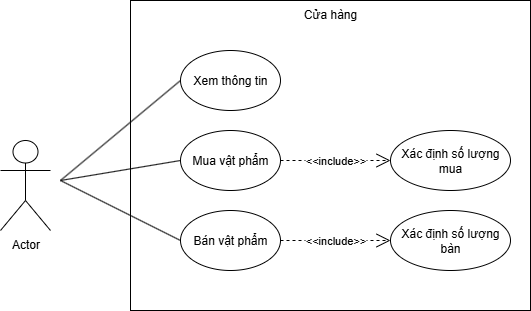
\includegraphics[width=14cm]{Images/ShopUCD.png}
	\vspace{0.5cm}
	\caption{Usecase Diagram Cửa hàng của Game}
\end{figure}
\begin{center}
	\begin{tabular}{|l|p{12cm}|}
		\hline
		ID and Name & UC2: Cửa hàng \\
		\hline
		Actor  & Người chơi \\
		\hline
		Description  & Use-case này chỉ các khả năng người chơi khi truy cập trang cửa hàng\\
		\hline
		Trigger  & Người chơi nhấn chuột trái vào nút mở Cửa hàng.\\
		\hline
		Pre-conditions & Người chơi hiện đang ở màn hình chính hoặc ở màn hình chọn màn chơi\\
		\hline
		Post-conditions & Người chơi mua bán vật phẩm thành công\\
		\hline
		\multirow{2}{*}{Normal flow}      &\qquad 1. Người chơi xem thông tin, bao gồm thông tin của các vật phẩm của cửa hàng, các vật phẩm mà người chơi hiện có và số xu của người chơi.\\
		&\qquad 2. Người chơi ấn vào vật phẩm mà người chơi cần mua hoặc vật phẩm trong kho đồ mà người chơi muốn bán\\
		&\qquad 3. Người chơi chọn số lượng cần mua/bán và xác nhận\\
		&\qquad 4. Người chơi ấn Đóng, kết thúc usecase\\
		\hline
		Alternative flow  & \qquad A1. Sau bước 3, người chơi có thể quay trở lại bước 1 để có thể tiếp tục truy cập cửa hàng\\
		&\qquad A2. Tại bước 3, Người chơi huỷ xác nhận mua vật phẩm, quay trở lại bước 1.\\
		\hline
		Exceptions  & E1. Tại bước 1, người chơi ấn nút đóng để đóng kho đồ. Use-case dừng lại\\
		\hline
	\end{tabular}
\end{center}
\subsubsection{Chọn màn chơi}
Use-case cho chức năng chọn màn chơi
\begin{figure}[H]
	\centering
	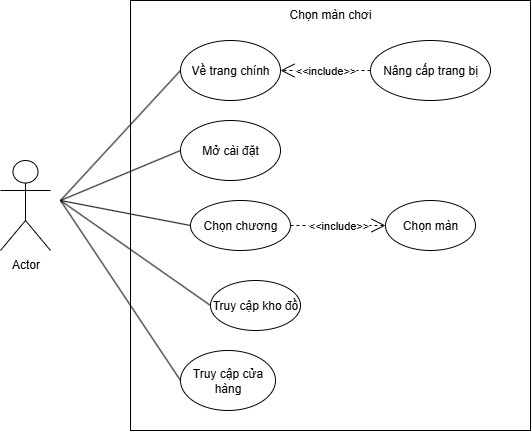
\includegraphics[width=14cm]{Images/LevelChooseUCD.png}
	\vspace{0.5cm}
	\caption{Usecase Diagram Chọn màn chơi}
\end{figure}
\begin{center}
	\begin{tabular}{|l|p{12cm}|}
		\hline
		ID and Name & UC3: Chọn màn chơi \\
		\hline
		Actor  & Người chơi \\
		\hline
		Description  & Use-case này chỉ các khả năng người chơi khi người chơi đang ở màn hình chọn màn chơi\\
		\hline
		Trigger  & Người chơi nhấn chuột trái vào nút Play ở trang chủ.\\
		\hline
		Pre-conditions & Người chơi hiện đang ở màn hình chính.\\
		\hline
		Post-conditions & Người chơi vào màn mà mình cần chơi\\
		\hline
		\multirow{2}{*}{Normal flow}      &\qquad 1. Người chơi chọn chương (hoặc vùng đất) đã mở khoá mà người chơi muốn chơi.\\
		&\qquad 2. Một danh sách các màn chơi của vùng đất mà người chọn được hiện ra. Người chơi nhấn chọn màn chơi đã mở khoá mà người chơi muốn chơi.\\
		&\qquad 3. Người chơi vào chơi màn chơi, kết thúc use-case\\
		\hline
		Alternative flow  & \qquad A1. Tại bước 1, người chơi có thể ấn nút Back để trở lại màn hình chính\\
		&\qquad A2. Tại bước 2, người chơi có thể quay trở lại để trở lại màn hình chọn chương (vùng đất)\\
		&\qquad A3. Tại bước 1 và 2, người chơi có thể mở kho đồ, cửa hàng hoặc cài đặt bằng các nút tương ứng\\
		\hline
		Exceptions  & \_\\
		\hline
	\end{tabular}
\end{center}

\subsubsection{Chơi màn chơi}
Use-case cho màn chơi
\begin{figure}[H]
	\centering
	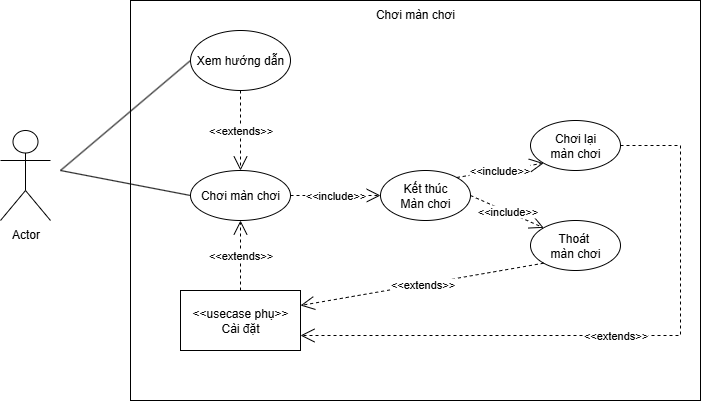
\includegraphics[width=14cm]{Images/PlayLevelUCD.png}
	\vspace{0.5cm}
	\caption{Usecase Diagram Chơi màn chơi}
\end{figure}
\begin{center}
	\begin{tabular}{|l|p{12cm}|}
		\hline
		ID and Name & UC4: Chơi màn chơi \\
		\hline
		Actor  & Người chơi \\
		\hline
		Description  & Use-case này chỉ các khả năng người chơi khi người chơi đang ở trong màn chơi\\
		\hline
		Trigger  & Người chơi chọn mở màn chơi từ danh sách màn chơi ở vùng đất mà người chơi đã chọn ở màn hình chọn màn chơi.\\
		\hline
		Pre-conditions & Người chơi mở khoá được màn chơi mình chọn\\
		\hline
		Post-conditions & Sau khi người chơi kết thúc màn chơi (thắng hoặc thua), người chơi có thể thoái về màn hình chọn màn chơi hoặc chơi lại màn. 
		\begin{itemize}
			\item Nếu người chơi thắng, người chơi được các phần thưởng người chơi đã thu thập được trong màn chơi (bao gồm xu, điểm kinh nghiệm, các món vật phẩm đã thu thập).
			\item Nếu người chơi thua, người chơi mất tất cả phần thưởng đã thu thập trong màn chơi.
		\end{itemize}\\
		\hline
		\multirow{2}{*}{Normal flow}      &\qquad 1. Khi vào màn chơi, người chơi chơi màn chơi mà người chơi đã chọn\\
		&\qquad 2. Sau khi người chơi kết thúc màn chơi với điều kiện thắng hoặc thua, trò chơi tính toán kết quả và hiển thị thông báo. Nếu thắng thì hiển thị những phần thưởng người chơi được nhận vì đã hoàn thành màn chơi.\\
		&\qquad 3. Người chơi nhấn chọn thoát màn chơi\\
		&\qquad 4. Use-case kết thúc, người chơi trở lại màn hình chọn màn chơi\\
		\hline
		Alternative flow  & \qquad A1. Tại bước 1, người chơi có thể ấn nút Cài đặt để vào cài đặt\\
		&\qquad A2. Tại bước 1,  người chơi có thể xem hướng dẫn với nhiều cách khác nhau \begin{itemize}
			\item Hướng dẫn tự bật lên
			\item Người chơi ấn vào nút hướng dẫn để hộp thoại hướng dẫn bật lên
		\end{itemize} Người chơi ấn nút đóng để đóng hướng dẫn và tiếp tục bước 1\\
		&\qquad A3. Tại bước 3, người chơi ấn chọn chơi lại để chơi màn chơi. Hệ thống đưa người chơi quay trở lại bước 1 với màn chơi không thay đổi và bắt đầu lại từ đầu\\
		\hline
		Exceptions  & \qquad E1. Tại bước A1, người chơi có thể ấn chơi lại hoặc thoát màn chơi giữa chừng. Sau khi xác nhận, hệ thống xử thua người chơi và bước xử lý tiếp theo tương ứng với các hành động người chơi đã thực hiện như sau: \begin{itemize}
			\item Nếu người chơi thoát màn chơi, người chơi được đưa về màn hình chọn màn chơi, kết thúc use-case
			\item Nếu người chơi chơi lại, Hệ thống đưa người chơi quay trở lại bước 1 với màn chơi không thay đổi và bắt đầu lại từ đầu.
		\end{itemize}\\
		\hline
	\end{tabular}
\end{center}

\subsubsection{Cài đặt}
Use-case cho chức năng Cài đặt
\begin{figure}[H]
	\centering
	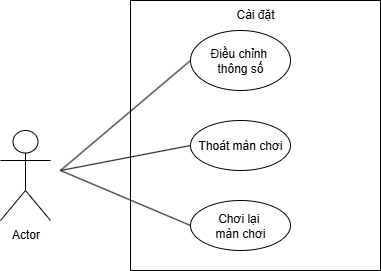
\includegraphics[width=14cm]{Images/SettingUCD.png}
	\vspace{0.5cm}
	\caption{Usecase Diagram Cài đặt}
\end{figure}
\begin{center}
	\begin{tabular}{|l|p{12cm}|}
		\hline
		ID and Name & UC5: Cài đặt \\
		\hline
		Actor  & Người chơi \\
		\hline
		Description  & Use-case này chỉ các khả năng người chơi khi người chơi truy cập vào cài đặt\\
		\hline
		Trigger  & Người chơi nhấn chuột trái vào nút Cài đặt\\
		\hline
		Pre-conditions & Nút Cài đặt trong trạng thái có nhấn được.\\
		\hline
		Post-conditions & Người chơi hoàn thành hiệu chỉnh thông số cài đặt\\
		\hline
		\multirow{2}{*}{Normal flow}      &\qquad 1. Người chơi điều chỉnh thông só cài đặt.\\
		&\qquad 2. Người chơi nhấn nút đóng, kết thúc use-case\\
		\hline
		Alternative flow  & \_\\
		\hline
		Exceptions  & \qquad E1. Trong bước 2, Người chơi nhấn nút thoát màn chơi và xác nhận chọn thoát, hệ thống xử thua, đưa người chơi về màn hình chọn màn chơi và kết thúc use-case\\
		&\qquad E2. Trong bước 2, Người chơi nhấn nút chơi lại màn chơi và xác nhận chọn chơi lại, hệ thống xử thua, đưa người chơi vào chơi lại màn chơi, kết thúc use-case\\
		\hline
	\end{tabular}
\end{center}
